\begin{frame}
\frametitle{Goal of measurements}
\begin{itemize}
	\item Conducting performance evaluations of \textbf{ringmap} capturing stack
		\begin{itemize}
			\item CPU-Load and packet loss during capturing\newline
		\end{itemize}
	\item Benchmarking: \textbf{generic} vs. \textbf{ringmap}
\end{itemize}
\end{frame}

%\begin{frame}
%\frametitle{What is measured ?}
%\textbf{packet loss} and \textbf{CPU-Load} as a function of :\newline
%\begin{itemize}
%	\item Traffic parameters
%		\begin{itemize}
%			\item packet size
%			\item bit-rate and packet-rate
%		\end{itemize}
%
%\color{gray}
%	\item  Hardware components
%		\begin{itemize}
%\color{gray}
%			\item PCI vs. PCI-Express
%			\item Number of CPUs
%		\end{itemize}
%	\item Driver parameters
%		\begin{itemize}
%\color{gray}
%			\item Size of packet puffers 
%			\item etc\ldots
%		\end{itemize}
%\end{itemize}
%\normalcolor
%\end{frame}
%
%\subsection*{Testbed}

\begin{frame}
\frametitle{Testbed}
\begin{center}
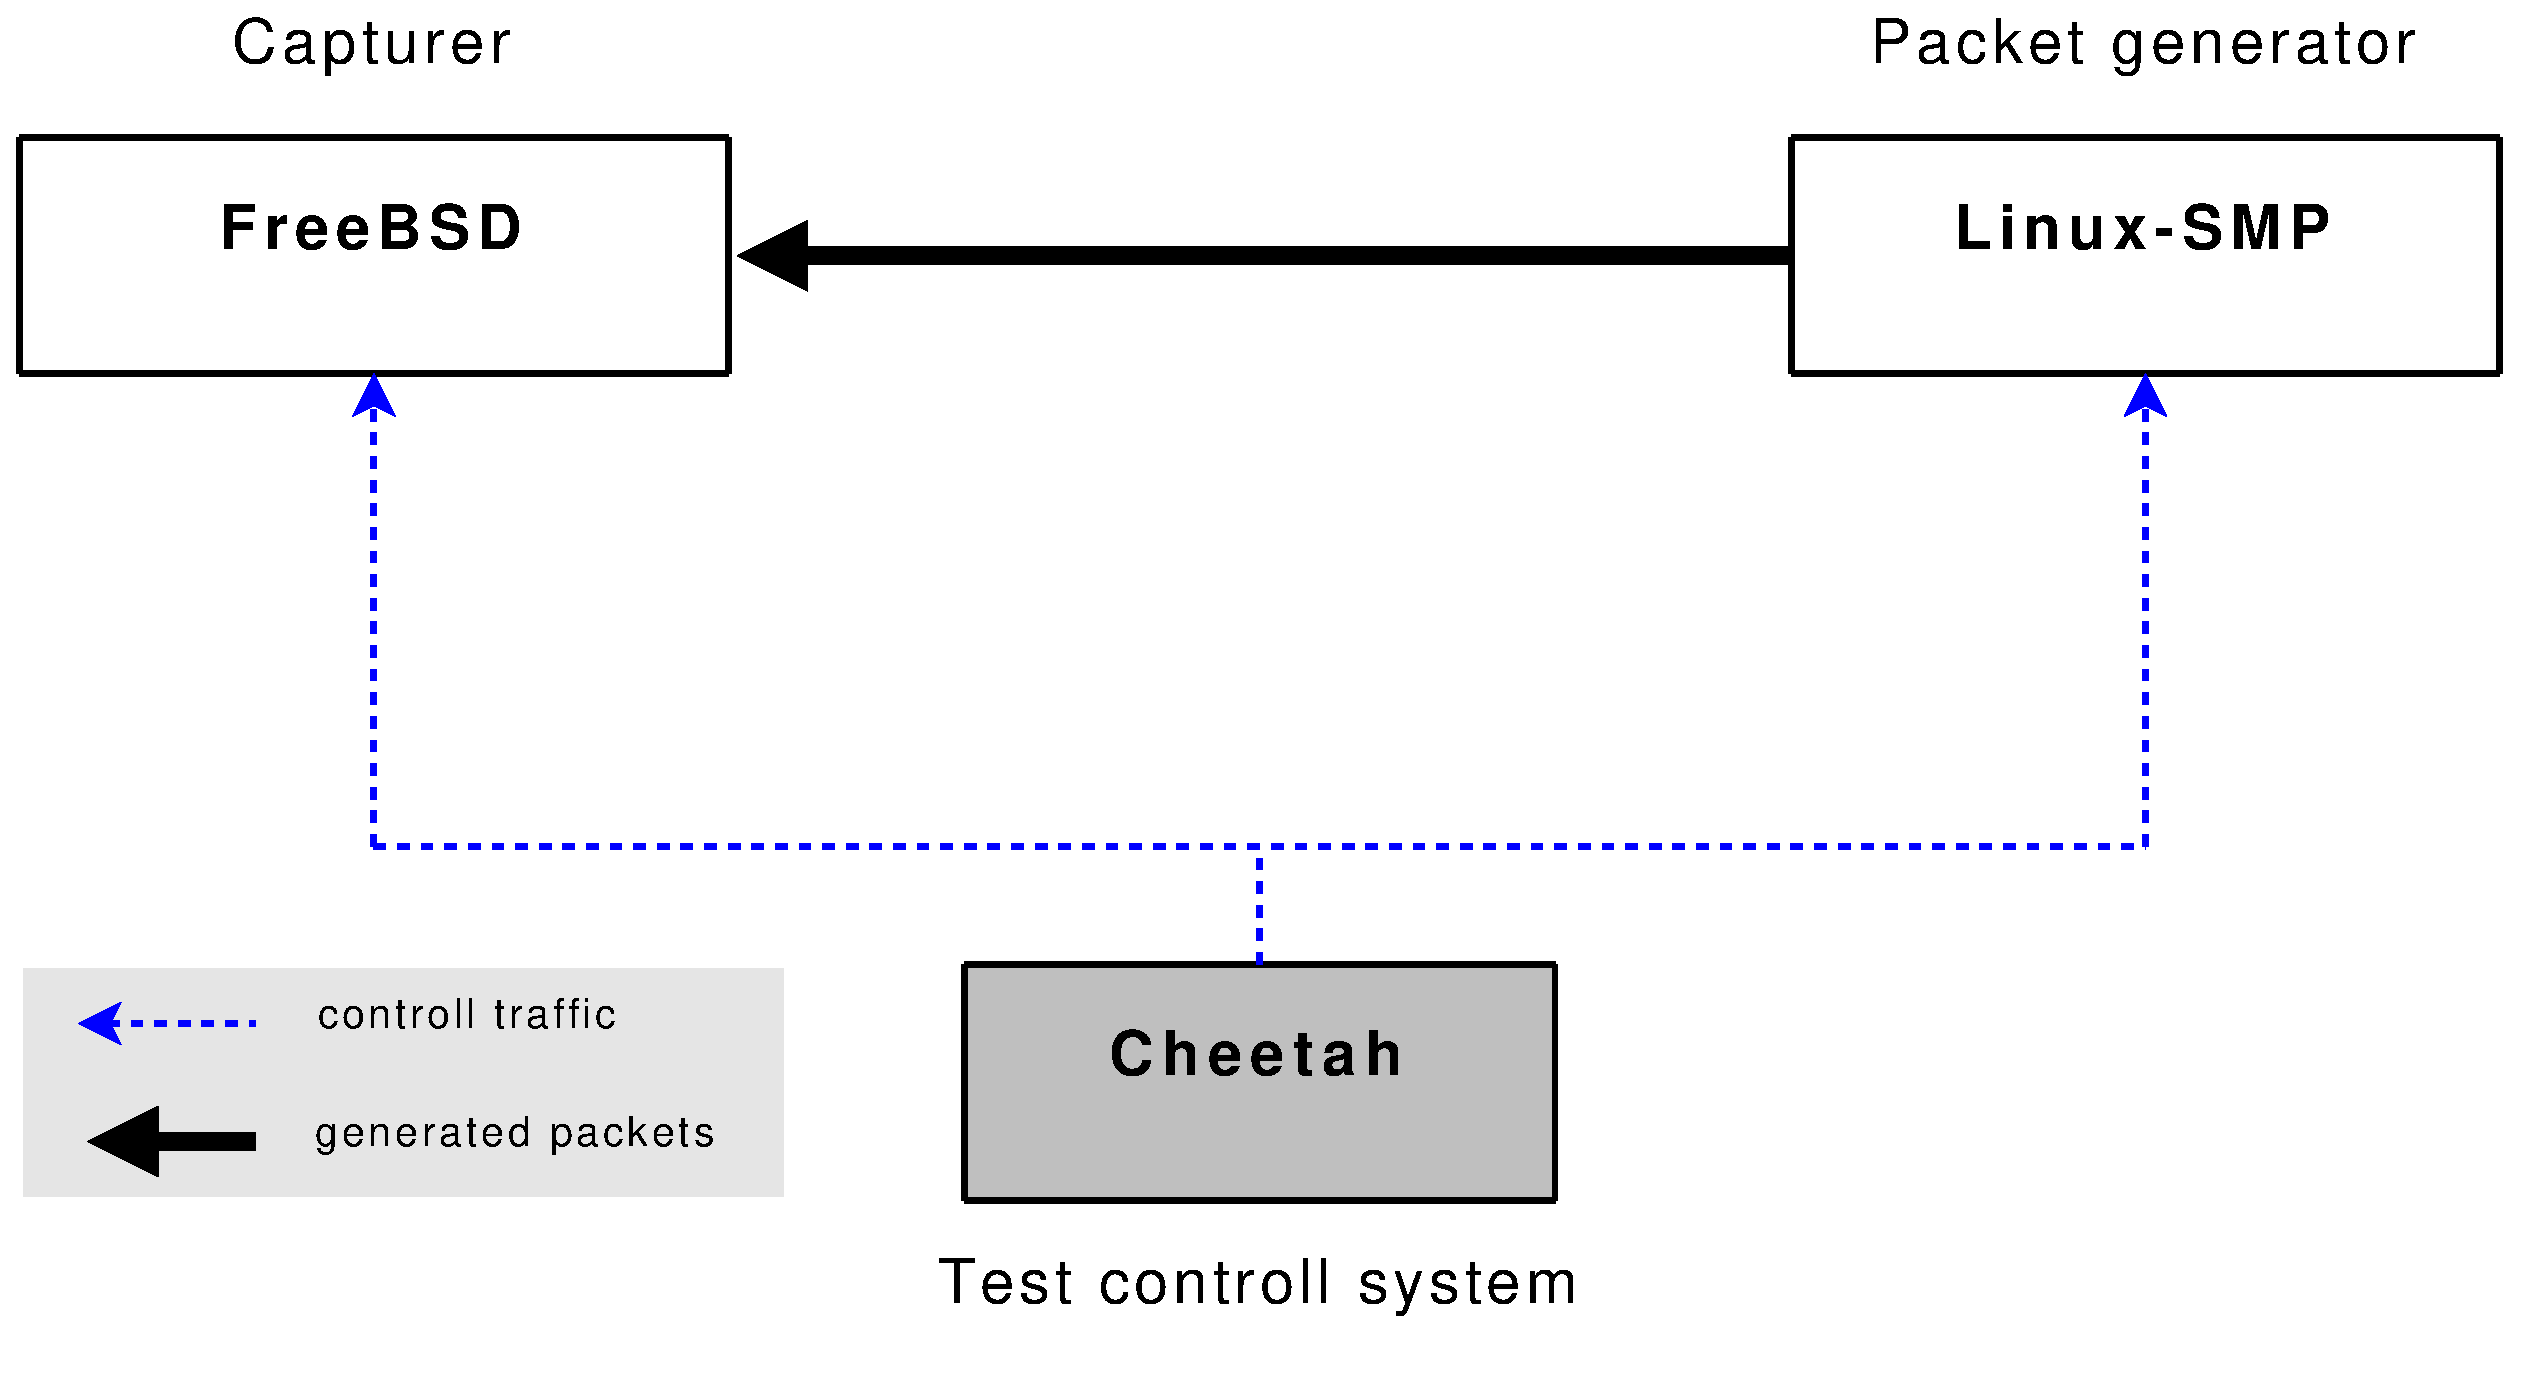
\includegraphics [height=0.68\textheight]{pics/Messaufbau}
\end{center}
\end{frame}

\begin{frame}
\frametitle{Measurement setup}
\textbf{Traffic generation}
\begin{itemize}
	\item Linux Kernel Packet Generator (\emph{pktgen})
		\begin{itemize}
			\item generates network packets at very high speed with different: 
				\begin{itemize}
					\item packet sizes
					\item bit-rate and packet-rate
				\end{itemize}
		\end{itemize}
\end{itemize}
\textbf{Capturing}
\begin{itemize}
	\item \textbf{ringmap} and \textbf{generic} stacks
	\item Libpcap-application
		\begin{itemize}
			\item accessing packets through call \emph{pcap\_loop()}
			\item counting the captured packets
		\end{itemize}
\end{itemize}
\end{frame}

%\begin{frame}
%\frametitle{Experiment parameters}
%For each experiment, data streams are generated with different parameters:
%\begin{itemize}
%	\item Constant parameters: 
%		\begin{itemize}
%			\item Packet size
%				\begin{itemize}
%					\item 64, 200, 300, 700, 1500
%				\end{itemize}
%		\end{itemize}
%	\item Variable parameters: 
%		\begin{itemize}
%			\item bit-rate 
%				\begin{itemize}
%					\item  $ < 1GBit/sec$
%				\end{itemize}
%		\end{itemize}
%\end{itemize}
%
%\end{frame}

\begin{frame}
\frametitle{Calculation of results}
\begin{itemize}
	\item System load
		\begin{itemize}
			\item Percentage proportion of time the CPU spent in system mode
			\item Interrupt load is not considered
				\begin{itemize}
					\item because of interrupt-throttling it is always constant for \textbf{generic} and \textbf{ringmap}
				\end{itemize}
			\item $syst = 1 - intr - user - nice - idle$\newline
		\end{itemize}
	\item Packet loss
		\begin{itemize}
			\item Difference between generated and captured packets
			\item $Packets_{loss} = Packets_{send} - Packets_{received}$
		\end{itemize}
\end{itemize}
\end{frame}

\subsection*{Testing sequence}
%%%%%%%%%%%%%%%%%%%%%%%%%%%%%%%%%%%%%%%%%%%%%%%%%%%%%%%%%%%%%%%%%%%
\begin{frame}
\frametitle{Testing sequence}
\begin{enumerate}
	\item Login to the capturer to 
		\begin{itemize}
			\item start of capturing 
			\item start of system load measurement applications 
		\end{itemize}
	\item Login to the Packet-Generator to 

	\begin{itemize}
		\item generate traffic with:
				\begin{itemize}
					\item a certain number of packets
					\item a certain bit-rate and packet-rate
				\end{itemize}
	\end{itemize}

	\item Login to the capturer to 
		\begin{itemize}
			\item stop capturing- and measurement-applications
		\end{itemize}
	\item Storing of measured values
\end{enumerate}
\begin{itemize}
	\item Each experiment is repeated five times
	\item The mean and standard deviation is calculated
\end{itemize}
\end{frame}

%\subsection*{Probleme bei Experimenten}
%%%%%%%%%%%%%%%%%%%%%%%%%%%%%%%%%%%%%%%%%%%%%%%%%%%%%%%%%%%%%%%%%%%%
%\begin{frame}
%\frametitle{Problems arose in experiments }
%\begin{itemize}
%	\item Instability of  Linux Kernel Packet Generator
%		\begin{itemize}
%			\item often kernel panics
%			\item [$\Rightarrow$] therefore max. $15000000 pkts$ per experiment\newline
%		\end{itemize}
%	\item Impossible to generate traffic with any packet- or bit-rate
%		\begin{itemize}
%			\item because of Interrupt-Throttling
%			\item [$\Rightarrow$] therefore only certain measurement points \newline
%		\end{itemize}
%	\item Flow-Control
%		\begin{itemize}
%			\item limits the rate of generated traffic
%			\item [$\Rightarrow$] therefore must be switched off
%		\end{itemize}
%\end{itemize}
%\end{frame}
